\documentclass[11pt]{beamer}

% Font-related packages
\usepackage{lmodern}
\usepackage{textcomp}

\usepackage[export]{adjustbox}

% Table-related packages
\usepackage{multirow}
\usepackage{booktabs}
\usepackage{hhline}
\usepackage[caption=false]{subfig}

% Graphics packages
\usepackage{tikz}

% Figures' path
\graphicspath{{images/}}

\usetheme{Pittsburgh}

% Add Logos
\addtobeamertemplate{headline}{}{%
\begin{tikzpicture}[remember picture,overlay]
\node at([shift={(.05\paperwidth,0.6)}]current page.south west) {
\includegraphics[height=.5cm,width=.5cm]{HotelsLogo.png}};
\node at([shift={(.9\paperwidth,0.6)}]current page.south west) {
\includegraphics[height=.5cm,width=.5cm]{EdinburghLogo.png}};
\node at([shift={(.95\paperwidth,0.6)}]current page.south west) {
\includegraphics[height=.5cm,width=.5cm]{AristotleLogo.png}};
\end{tikzpicture}}
  
\title{Summarizing Software API Usage Examples Using Clustering Techniques}

\author{N.~Katirtzis\inst{1,2} \and T.~Diamantopoulos\inst{3} \ and C.~Sutton\inst{2}}

\institute[]
{
  \inst{1}%
  Hotels.com
  \and
  \inst{2}%
  School of Informatics\\
  University of Edinburgh, Edinburgh, UK
  \and
  \inst{3}%
  Electrical and Computer Engineering Department\\
  Aristotle University of Thessaloniki, Thessaloniki, Greece\\
}

\date{21st International Conference on Fundamental Approaches to Software Engineering (\textit{FASE}), 2018}

\subject{Theoretical Computer Science}

\AtBeginSubsection[]
{
  \begin{frame}<beamer>{Outline}
    \tableofcontents[currentsection,currentsubsection]
  \end{frame}
}


\begin{document}

\begin{frame}
	\titlepage
\end{frame}

\subsection*{CLAMS}
\begin{frame}{\textbf{CL}ustering for \textbf{A}pi \textbf{M}ining of \textbf{S}nippets}
	\begin{exampleblock}{CLAMS}
		An approach for mining API usage examples from client code that lies between snippet and sequence mining methods, which ensures lower complexity and thus could apply more readily to other languages.
	\end{exampleblock}
	\begin{exampleblock}{Sample Snippet}
		\vspace{-5pt}
		\begin{figure}
			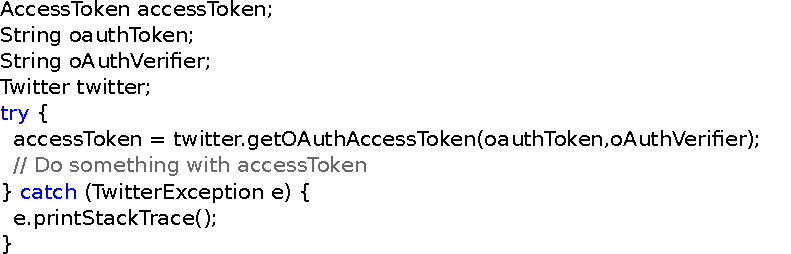
\includegraphics[scale=0.7, left]{HandwrittenExample}
		\end{figure}
		\vspace{-10pt}
	\end{exampleblock}
\end{frame}

\begin{frame}{Outline}
	\tableofcontents
\end{frame}

\section{Background}

\subsection{Introduction}

\begin{frame}{Introduction}{}
	\vspace{30pt}
	\begin{itemize}
		\item {
			Third-party libraries are used heavily during SDLC.
		}
		\item {
			Lack of proper documentation for the APIs of the libraries.
		}
		\item {
			Creating API usage examples is time-consuming.
		}
	\end{itemize}
	\begin{figure}
		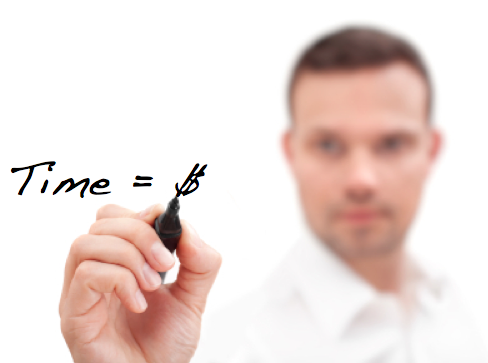
\includegraphics[scale=0.25]{Time}
	\end{figure}
\end{frame}

\subsection{Problem Statement}

\begin{frame}{Problem Statement}
	\begin{figure}
		
\includegraphics[scale=0.25]{TheProblem}
	\end{figure}
	\begin{block}{The Problem}{Automatically identify a set of patterns that characterize how an API is typically used from a corpus of client code (\textit{API usage mining}).}
	\end{block}
\end{frame}

\subsection{Related Work}

\begin{frame}{Related Work}{}
	\begin{itemize}
		\item {
			Systems that Output API Call Sequences\\
			\vspace{5pt}
			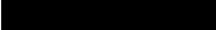
\includegraphics[scale=0.5]{SequenceOutput}
		}
		\item {
			Systems that Output Source Code Snippets\\
			\vspace{5pt}
			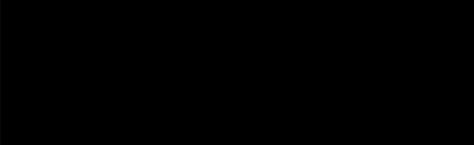
\includegraphics[scale=0.5]{SnippetOutput}
		}
	\end{itemize}
\end{frame}

\begin{frame}{Related Work}{Systems that Output API Call Sequences}
	\begin{itemize}
		\item {
			MAPO (frequent sequence mining, clustering)
		}
		\item {UP-Miner (clustering)
		}
		\item {PAM (probabilistic modeling)
		}
	\end{itemize}
	  
	\begin{alertblock}{Disadvantages}
		\begin{itemize}
			\item {
				API call sequences do not always describe important information like method arguments and control flow.
			}
			\item {The output cannot be directly included in one's code.
			}
		\end{itemize}
	\end{alertblock}
\end{frame}

\begin{frame}{Related Work}{Systems that Output Source Code Snippets}
	\begin{itemize}
		\item {
			eXoaDocs (clustering, program slicing)
		}
		\item {
			APIMiner (program slicing, association rules)
		}
		\item{
		      Buse and Weimer (path-sensitive data flow analysis, clustering, pattern abstraction)
		}
	\end{itemize}
	\begin{alertblock}{Disadvantages}
		\begin{itemize}
			\item{
			      Rely on detailed semantic analysis and semantic features which can make them more difficult to deploy to new languages.
			}
			\item {Limited source code summarization capabilities.
			}
		\end{itemize}
	\end{alertblock}
\end{frame}

\section{Methodology}

\subsection{The Concept}
\begin{frame}{The Concept}{}
	\begin{figure}
		
\includegraphics[scale=0.13]{TheConcept}
	\end{figure}
	\vspace{-25pt}
	\begin{block}{}{
			\begin{enumerate}
				\item
				      Cluster a large set of usage examples based on their API calls.
				\item Generate summarized versions for the top snippets of each cluster.
				\item Select the most representative snippet from each cluster, using a tree edit distance metric on the ASTs.
				\item Rank the snippets in descending order of support.
			\end{enumerate}}
	\end{block}
\end{frame}


\subsection{System Overview}

\begin{frame}{System Overview}{}
	\begin{figure}
		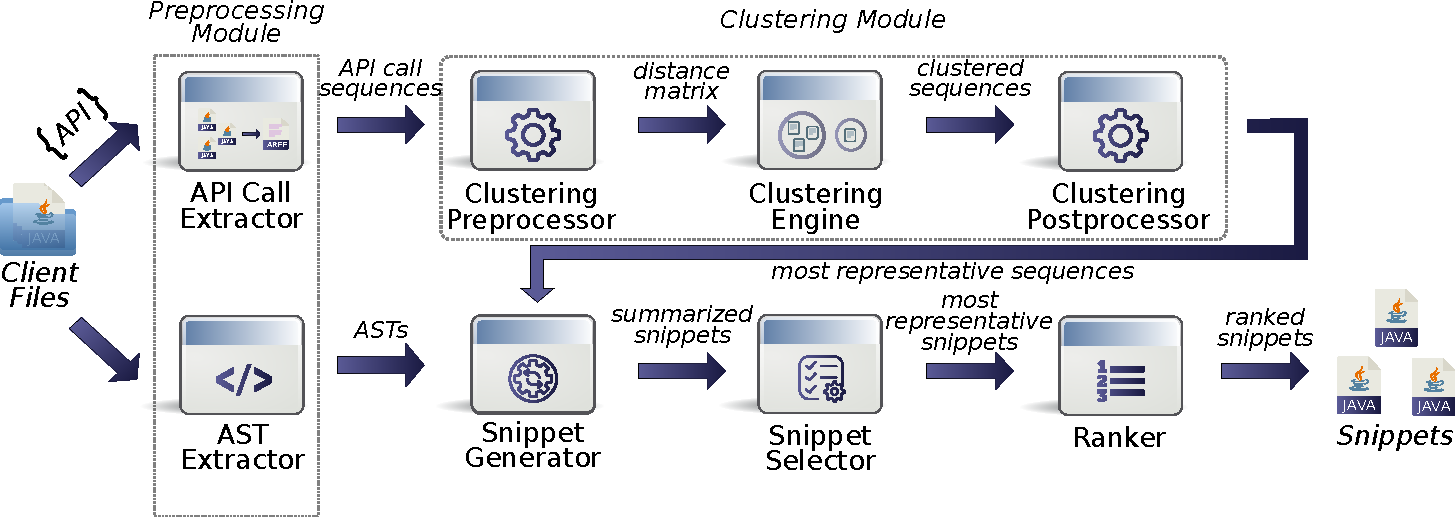
\includegraphics[scale=0.4]{CLAMSArchitecture}
	\end{figure}
	\begin{align*}
		\begin{array}{ll} 
		\textrm{Input}
		\end{array}                    & \Rightarrow 
		\bigg\{\begin{array}{ll}  
		\textrm{A set of Client Files} &             \\
		\textrm{API of the library}\\
		\end{array}\\
		\begin{array}{ll}  %
		\textrm{Output}
		\end{array}                    & \Rightarrow 
		\begin{array}{l}
		\textrm{A set of source code snippets} \\
		\end{array}
	\end{align*}
\end{frame}

\subsubsection*{Preprocessing Module}

\begin{frame}{Preprocessing Module}
	\vspace{-40pt}
	API Call Extractor
	\vspace{-5pt}
	\begin{align*}
		\begin{array}{ll} 
		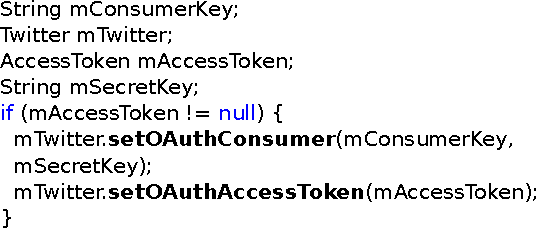
\includegraphics[scale=0.4]{SrcmlInput}
		\end{array} & \Rightarrow 
		\begin{array}{l}  
		
\includegraphics[scale=0.5]{CallExtractorOutput}
		\end{array}
	\end{align*}
	AST Extractor
	\vspace{-5pt}
	\begin{align*}
		\begin{array}{ll} 
		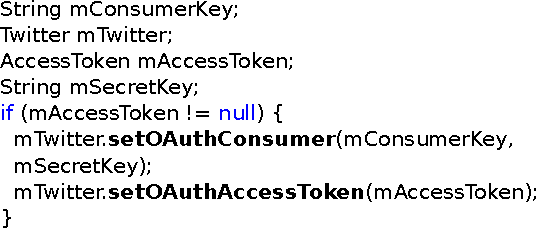
\includegraphics[scale=0.4]{SrcmlInput}
		\end{array} & \Rightarrow 
		\begin{array}{l}  
		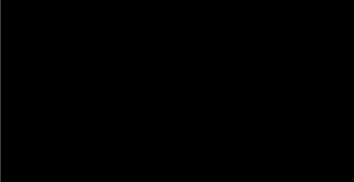
\includegraphics[scale=0.4]{SrcmlOutput}
		\end{array}
	\end{align*}
	\vspace{-60pt}
\end{frame}


\subsubsection*{Clustering Module}

\begin{frame}{Clustering Module}{Clustering Preprocessor}
	\begin{itemize}
		\item {
			We cluster at sequence level:
			\vspace{-10pt}
			\begin{figure}
				\def\thewidth{0.4\columnwidth}
				\centering
				\subfloat[][]{
					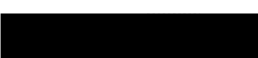
\includegraphics[width=\thewidth]{images/ClusterSnippet1}         
					}\hspace{5pt}
				\subfloat[][]{
					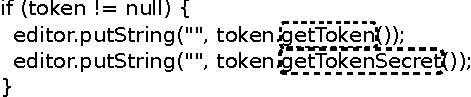
\includegraphics[width=\thewidth]{images/ClusterSnippet2}
				}
			\end{figure}
		}
		\item {
			Using the distance matrix which is based on the \textit{Longest Common Subsequence (LCS)} between any two API call sequences:
			\footnotesize	
			\begin{align}
				\centering                                                  
				LCS\_dist\left( S_1, S_2 \right) =                          
				1 - 2\cdot\frac{ \left| LCS\left( S_1, S_2 \right) \right|} 
				{\left| S_1 \right| + \left| S_2 \right|}                   
			\end{align}
			%
			\normalsize
			where $\left|S_1 \right|$ and $\left|S_2 \right|$ are the lengths of $S_1$ and $S_2$, and $\left|LCS\left( S_1, S_2 \right) \right|$ is the length of their LCS.
		}
	\end{itemize}
\end{frame}

\subsubsection*{Clustering Module}

\begin{frame}{Clustering Module}{Clustering Engine/Postprocessor}
	\begin{itemize}
		\item {
			Explores two different clustering algorithms:
			\begin{enumerate}  
				\item {
					\textcolor{red}{k-medoids} by Bauckhage.
				}
				\item {
					\textcolor{red}{HDBSCAN} by McInnes et al.
				}
			\end{enumerate}
		}
		\vspace{15pt}
		\item{
		      We then select multiple snippets for each cluster, this way retaining source code structure information, which shall be useful for selecting a single snippet.
		}  
	\end{itemize}
	 
\end{frame}

\subsubsection*{Snippet Generator}

\begin{frame}{Snippet Generator - Summarizer}
	\begin{figure}
		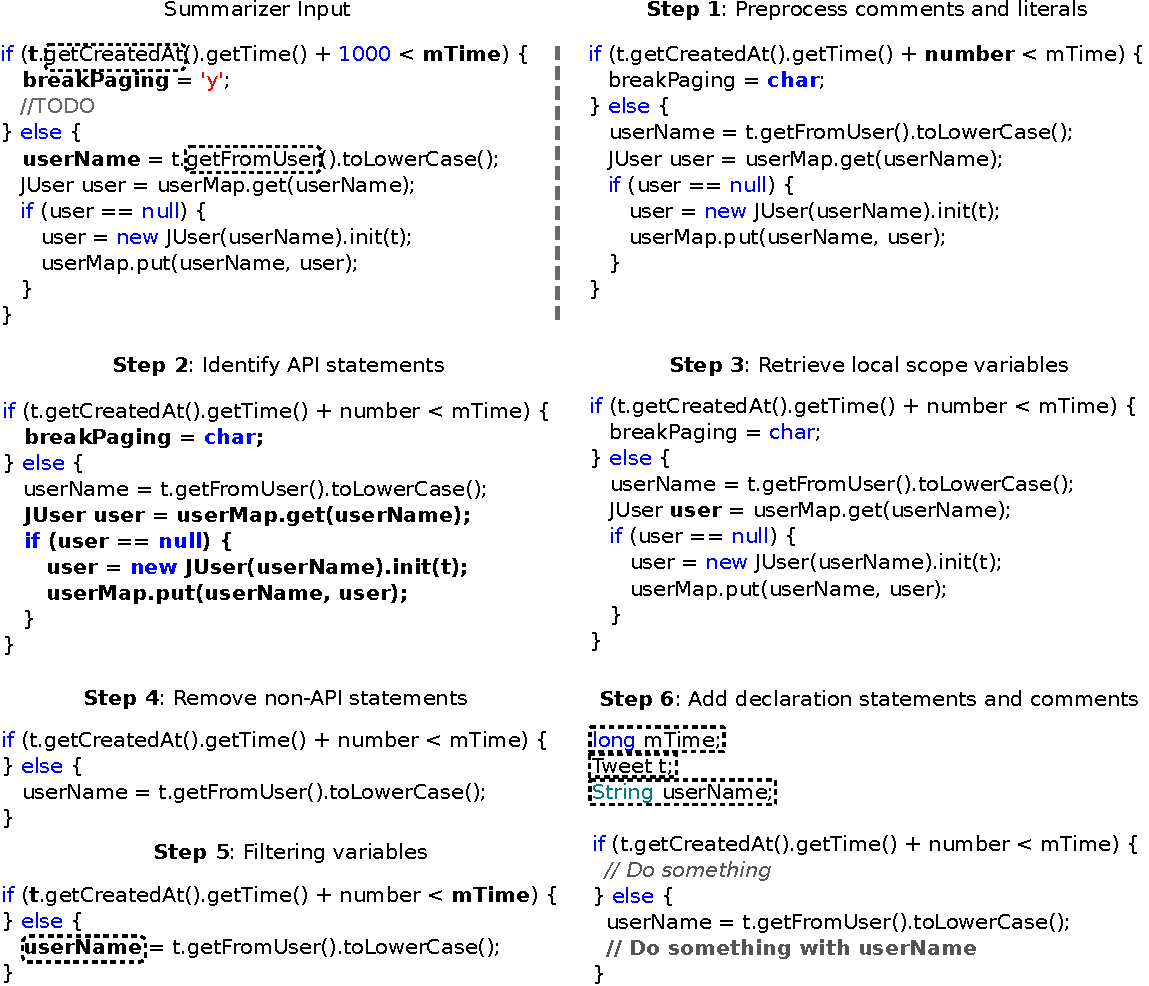
\includegraphics[scale=0.4]{SummarizerFlow}
	\end{figure}
\end{frame}

\subsubsection*{Snippet Selector}

\begin{frame}{Snippet Selector}
	\begin{block}{Goal}
		Select the most representative snippet of each cluster.
	\end{block}
	\begin{block}{Concept}
		\begin{itemize}
			\item{
			      Create a matrix for each cluster, which contains the distance between any two top snippets of the cluster.  
			}
			\item{
			      Use the APTED algorithm to compute the tree edit distance between any two snippets.
			}
			\item{
			      Select the snippet with the minimum sum of distances in each cluster's matrix.  
			}
		\end{itemize}
	\end{block}
\end{frame}

\subsubsection*{Ranker}

\begin{frame}{Ranker}
	\begin{block}{Goal}
		Rank the snippets in descending order of support.
	\end{block}
	\begin{block}{Concept}
		A client file supports a snippet if the API call sequence of the snippet is a subsequence of the sequence of that file.
	\end{block}
	\begin{exampleblock}{Example}
		The snippet with API call sequence:\\ 
		{[}\textcolor{red}{\textsf{twitter4j.Status.getUser}}, \textcolor{red}{\textsf{twitter4j.Status.getText}}]\\
		is supported by a client file with sequence:\\
		{[}\textsf{twitter4j.Paging.$<$init$>$}, \textcolor{red}{\textsf{twitter4j.Status.getUser}}, \textsf{twitter4j.Status.getId}, \textcolor{red}{\textsf{twitter4j.Status.getText}}, \textsf{twitter4j.} \textsf{Status.getUser}].
	\end{exampleblock}
\end{frame}

\subsection{Deploying to New Languages}

\begin{frame}{Deploying to New Languages}{}
	Our methodology can be easily deployed to additional programming languages.
	\begin{table}[!h]
		\setlength{\tabcolsep}{4pt}
		\centering
		\small
		\caption{Concept on which the CLAMS modules are based on.}
		\begin{tabular}{ll}
\toprule
\textbf{Module} & \textbf{Main Concept} \\
\midrule
\textbf{Preprocessing Module} & AST \\
\textbf{Clustering Module} & API Call Sequence \\
\textbf{Snippet Generator} & Statement/Control Flow\\
\textbf{Snippet Selector} & AST \\
\textbf{Ranker} & API Call Sequence \\
\bottomrule
\end{tabular}
	\end{table}
\end{frame}

\section{Evaluation}

\subsection{Evaluation Framework}

\begin{frame}{Evaluation Framework}{Dataset}
	\begin{table}[!h]
		\setlength{\tabcolsep}{4pt}
		\centering
		\small
		\caption{Summary of the evaluation dataset.}
		\label{tables:Dataset}
		\begin{tabular}{llrr}
\toprule
Project & Package Name & Client LOC & Example LOC\\
\midrule
Apache Camel & org.apache.camel & 141,454 & 15,256 \\
Drools & org.drools & 187,809 & 15,390 \\
Restlet Framework & org.restlet & 208,395 & 41,078 \\
Twitter4j & twitter4j & 96,020 & 6,560 \\
Project Wonder & com.webobjects & 375,064 & 37,181 \\
Apache Wicket & org.apache.wicket & 564,418 & 33,025 \\
\bottomrule
\end{tabular}
	\end{table}
\end{frame}

\begin{frame}{Evaluation Framework}{Research Questions}
	\begin{figure}[ht]
		\centering
		\small
		\renewcommand{\arraystretch}{1.075}
		\begin{tabular}{cp{0.75\textwidth}}
\toprule
\textbf{RQ1:} & How much more concise, readable, and precise with respect to handwritten examples are the snippets after summarization? \\
\textbf{RQ2:} & Do more powerful clustering techniques, that cluster similar rather than identical sequences, lead to snippets that more closely match handwritten examples? \\
\textbf{RQ3:} & Does our tool mine more diverse patterns than other existing approaches? \\
\textbf{RQ4:} & Do snippets match handwritten examples more than API call sequences? \\
\bottomrule
\end{tabular}
		\caption{Research Questions (RQs) to be evaluated.}
		\label{tables:RQs}
	\end{figure}
\end{frame}

\subsection{Evaluation Results}

\begin{frame}{Evaluation Results - RQ1}
	\textbf{RQ1: How much more \textcolor{red}{concise}, \textcolor{red}{readable}, and precise with respect to handwritten examples are the snippets after summarization?}
	  
	\begin{figure}
		\def\thewidth{0.4\columnwidth}
		\centering
		\subfloat[][]{
			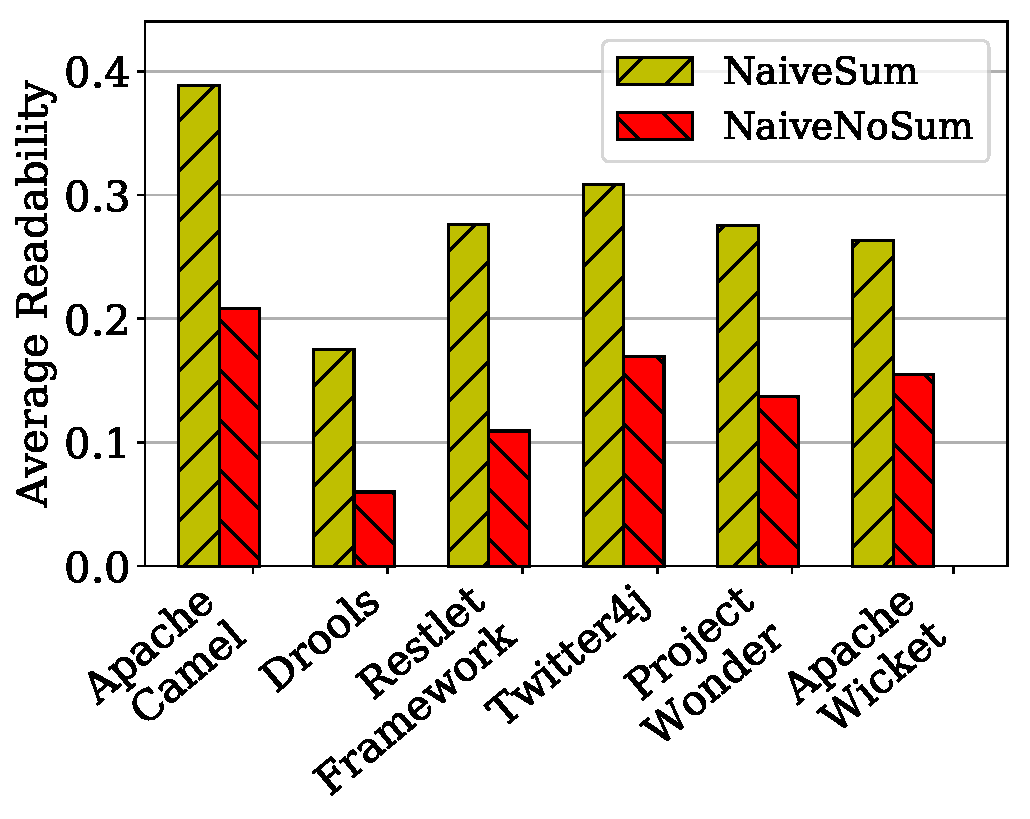
\includegraphics[width=\thewidth]{images/Exp1Readability} 
			\label{res:Exp1Readability}
		}
		\subfloat[][]{
			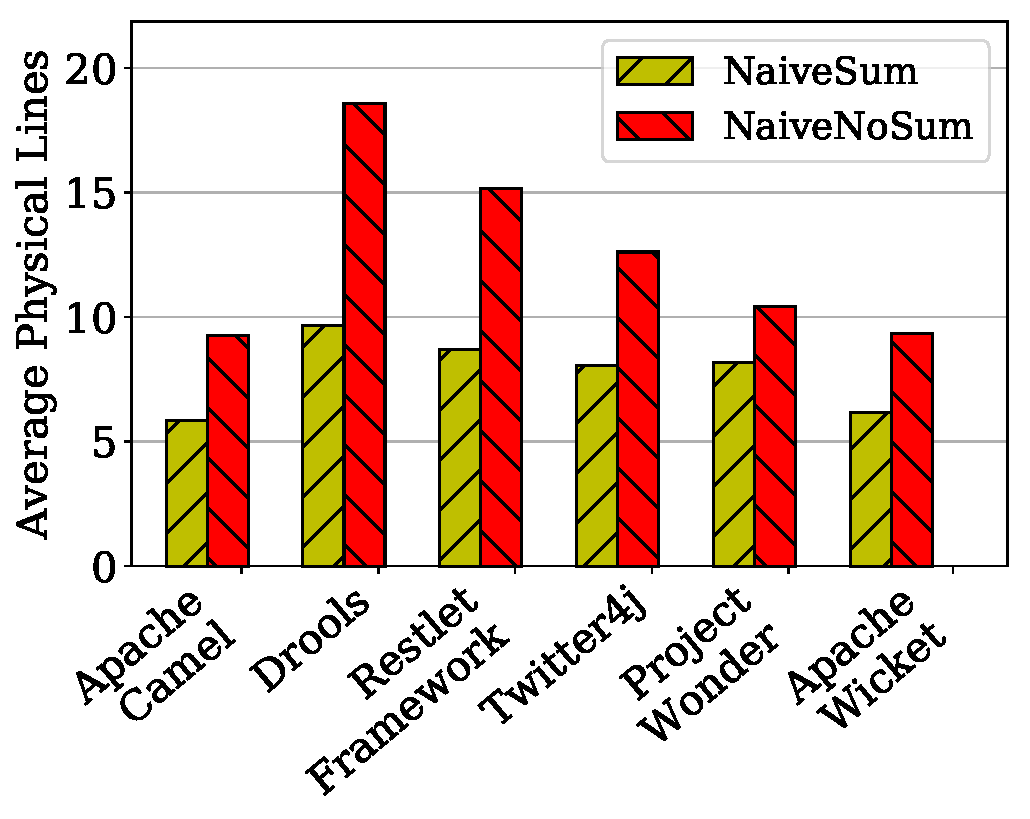
\includegraphics[width=\thewidth]{images/Exp1Plocs}
			\label{res:Exp1Plocs}
		}
		\caption[]{\subref{res:Exp1Readability}  average readability, and \subref{res:Exp1Plocs}  average PLOCs of the snippets, for each library, with (\textit{NaiveSum}) and without (\textit{NaiveNoSum}) summarization.}
	\end{figure}
\end{frame}

\begin{frame}{Evaluation Results - RQ1}
	\textbf{RQ1: How much more concise, readable, and \textcolor{red}{precise} with respect to handwritten examples are the snippets after summarization?}
	  
	\begin{figure}[ht]
		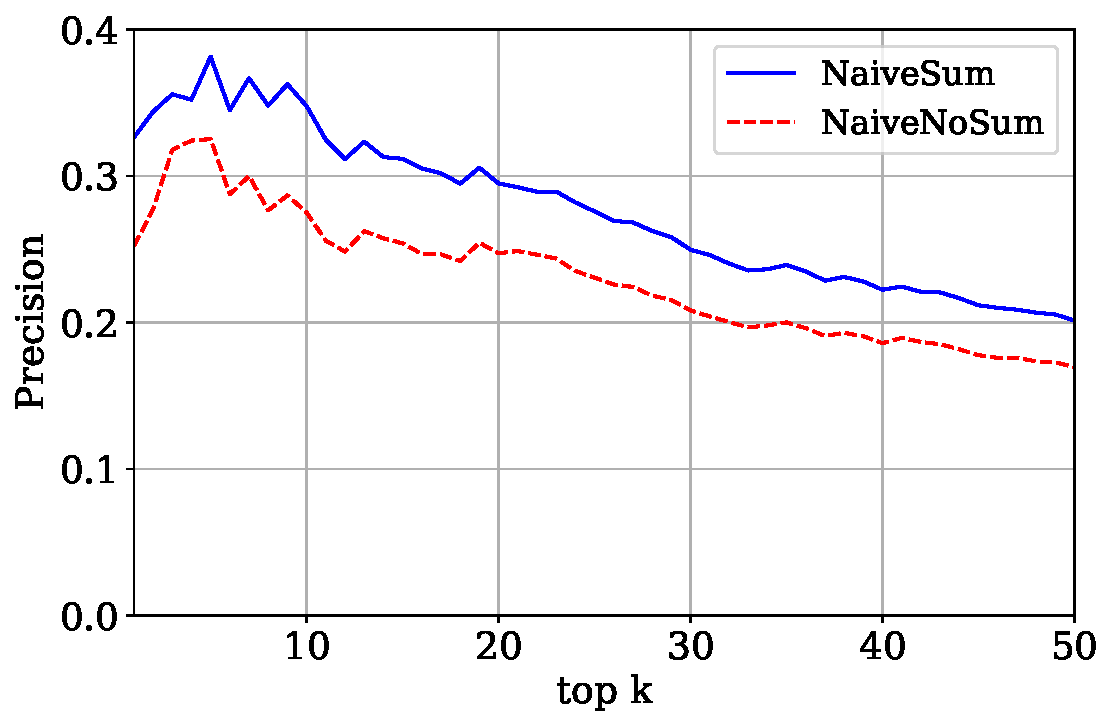
\includegraphics[scale=0.35]{images/Exp1Precision} 
		\caption[]{Precision at top $k$, with (\textit{NaiveSum}) or without (\textit{NaiveNoSum}) summarization using the top $50$ mined snippets.}
	\end{figure}
	  
\end{frame}

\begin{frame}{Evaluation Results - RQ2}
	\textbf{RQ2: Do more powerful clustering techniques, that cluster similar rather than identical sequences, lead to snippets that more closely match handwritten examples?}
	  
	\begin{figure}[ht]
		\centering
		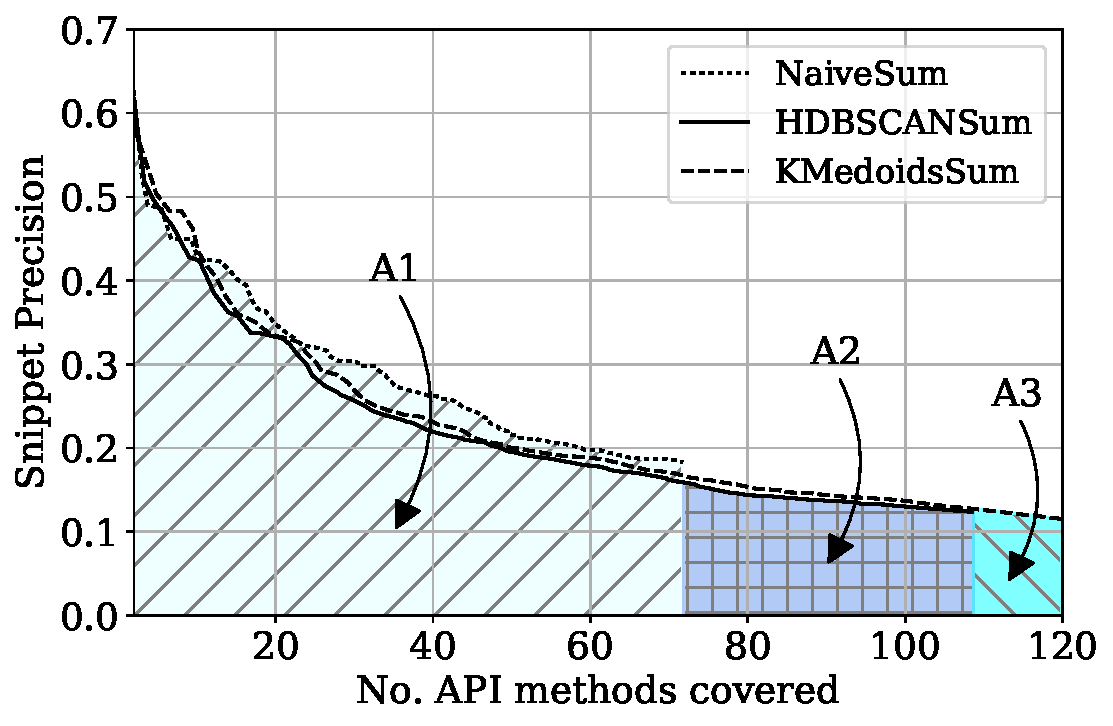
\includegraphics[scale=0.35]{images/Exp2InterpPrecCov} 
		\caption[]{Average interpolated snippet precision versus API coverage for three clustering algorithms, using the top $100$ mined snippets.}
	\end{figure}
\end{frame}

\begin{frame}{Evaluation Results - RQ3}
	\textbf{RQ3: Does our tool mine more diverse patterns than other existing approaches?}
	\begin{figure}
		\centering
		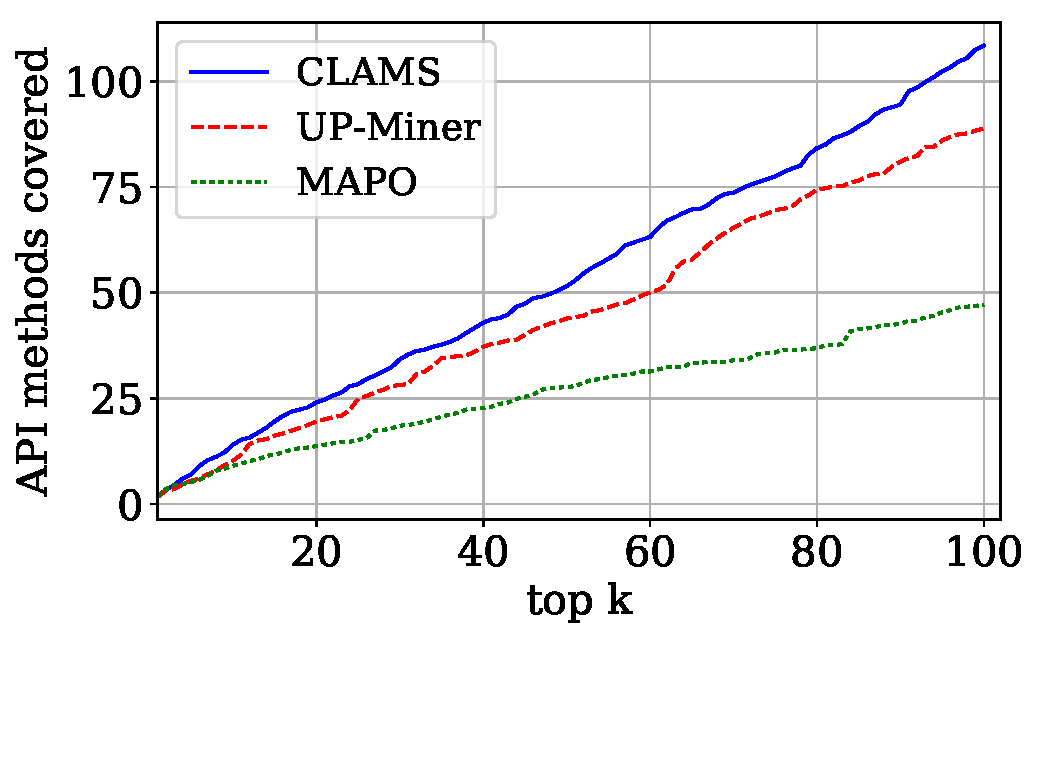
\includegraphics[scale=0.3]{images/Exp3CoverageAtk}
		\vspace{-20pt}
		\caption[]{Coverage in API methods achieved by CLAMS, MAPO, and UP-Miner on average, at top $k$, using the top 100 examples.}
	\end{figure}
\end{frame}

\begin{frame}{Evaluation Results - RQ4}
	\textbf{RQ4: Do source code snippets match handwritten examples more than API call sequences?}
	  
	\begin{figure}
		\centering
		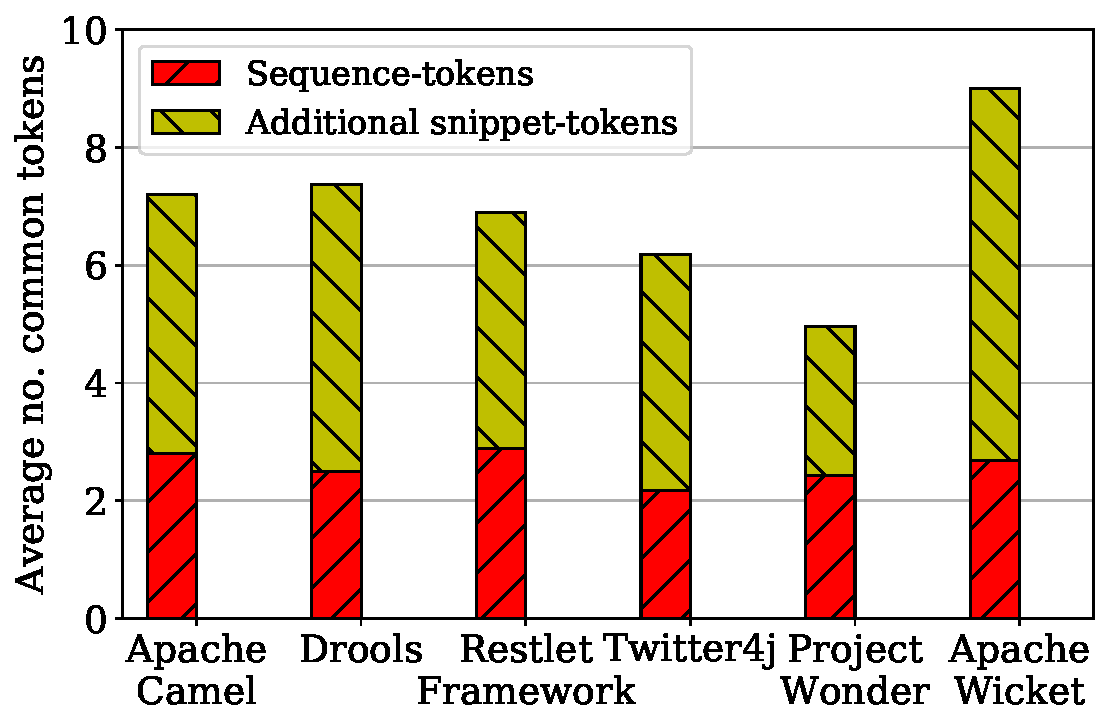
\includegraphics[width=0.525\columnwidth]{images/Exp4AdditInfo}
		\caption{Additional information revealed when mining snippets instead of sequences.}
		\label{res:Exp4AdditInfo}
	\end{figure}
\end{frame}

\begin{frame}{Evaluation Results - RQ4}
	\textbf{RQ4: Do source code snippets match handwritten examples more than API call sequences?}
	  
	\begin{figure}
		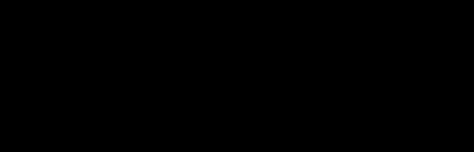
\includegraphics[scale=0.56]{MatchedExample}
		\caption{Example snippet matched to handwritten example. Sequence-tokens are encircled and additional snippet-tokens are highlighted in bold.}
	\end{figure}
\end{frame}


\begin{frame}{Applying CLAMS to the industry}
	\begin{figure}
		
\includegraphics[scale=0.2]{HappyCustomers}
	\end{figure}
	\vspace{-10pt}
	\begin{itemize}
		\item {
			We conducted a pilot user survey at a team of Java developers at Hotels.com which received encouraging feedback:
		}
	\end{itemize}
	\begin{quote}
		Developer 1: The system generates clear and concise snippets which would be easy to follow and useful when using an API you are unfamiliar with.
	\end{quote}
	\begin{quote}
		Developer 2: The system is great and I think it would be very useful particularly in discovering clients of our APIs!
	\end{quote}
\end{frame}

\begin{frame}{Applying CLAMS to the industry}
	\begin{itemize}
		\item {
			We applied CLAMS at Hotels.com and developed an internal method-based search engine which can be used for API documentation purposes.
		}
	\end{itemize}
	\begin{figure}
		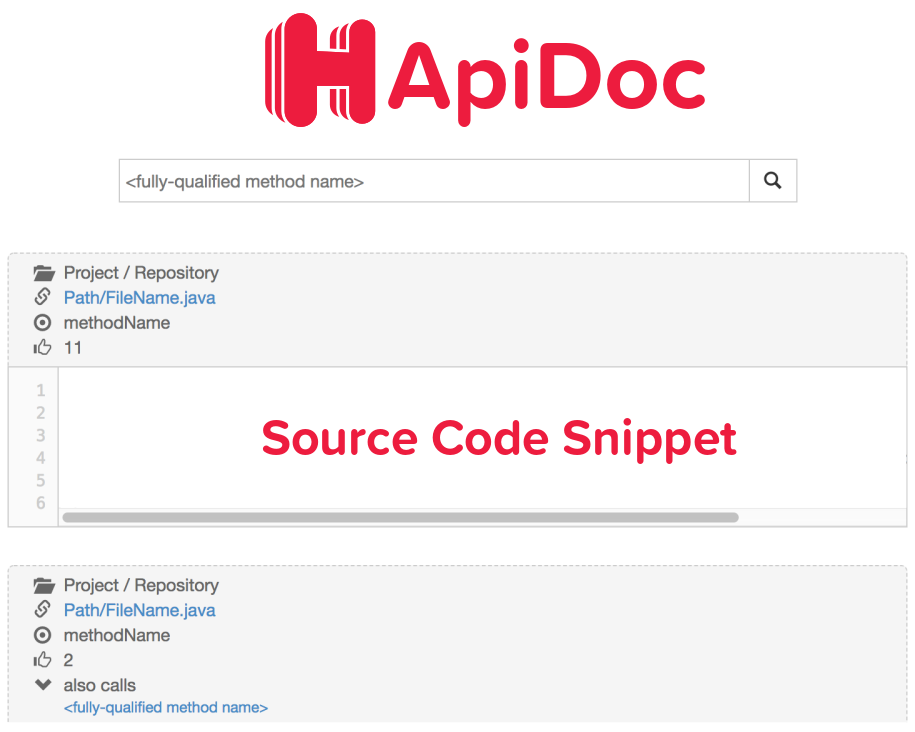
\includegraphics[scale=0.18]{HApiDocScreenshot}
	\end{figure}
\end{frame}

% All of the following is optional and typically not needed. 
\subsection<presentation>*{For Further Reading}

\begin{frame}
	\frametitle<presentation>{Resources}
	    
	\begin{thebibliography}{3}
		    
		\setbeamertemplate{bibliography item}[online]
		\bibitem{ClamsWebsite}
		CLAMS Website
		\newblock {\em \href{https://mast-group.github.io/clams/}{\beamergotobutton{https://mast-group.github.io/clams/}}}
		    
		\setbeamertemplate{bibliography item}[online]
		\bibitem{ClamsSurvey}
		CLAMS User Survey at Hotels.com
		\newblock {\em \href{https://mast-group.github.io/clams/user-survey/}{\beamergotobutton{https://mast-group.github.io/clams/user-survey/}}}
		    
		\setbeamertemplate{bibliography item}[online]
		\bibitem{ClamsGitHub}
		CLAMS Source Code
		\newblock {\em \href{https://github.com/mast-group/clams}{\beamergotobutton{https://github.com/mast-group/clams}}}
	\end{thebibliography}
\end{frame}

\end{document}
